% ============================================================
%  Relatório de Avaliação de Impacto Causal — DEAMs 24h Brasil
%  Estilo: academic-corporate (Journal of Investing / Factor Archives)
%  Compilar com: pdflatex -shell-escape deam24h_relatorio.tex
% ============================================================
\documentclass[twocolumn, 10pt]{article}

% ── Codificação e língua ────────────────────────────────────
\usepackage[utf8]{inputenc}
\usepackage[T1]{fontenc}
\usepackage[brazil]{babel}

% ── Fontes ─────────────────────────────────────────────────
\usepackage{lmodern}
\usepackage{helvet}           % fonte sans-serif para títulos

% ── Layout ─────────────────────────────────────────────────
\usepackage[
  top=2.0cm, bottom=2.2cm,
  left=1.6cm, right=1.6cm,
  columnsep=0.7cm
]{geometry}
\usepackage{microtype}
\usepackage[hyphens]{url}
\usepackage{setspace}
\setstretch{1.0}             % espaçamento entre linhas compacto (limite de páginas)
\emergencystretch=3em
\setlength{\parskip}{2pt}
\setlength{\parindent}{1.1em}

% ── Cabeçalho e rodapé ─────────────────────────────────────
\usepackage{fancyhdr}
\pagestyle{fancy}
\fancyhf{}
\renewcommand{\headrulewidth}{0.4pt}
\fancyhead[L]{\footnotesize\sffamily AVALIAÇÃO DE IMPACTO CAUSAL — DEAMs 24H}
\fancyhead[R]{\footnotesize\sffamily\thepage}
\fancyfoot[C]{\footnotesize\sffamily Projeto DEAM-BR \textbar{} Callaway \& Sant'Anna (2021)}

% ── Seções em sans-serif ───────────────────────────────────
\usepackage{titlesec}
\titleformat{\section}
  {\sffamily\bfseries\large}{\thesection}{0.6em}{}[\titlerule]
\titleformat{\subsection}
  {\sffamily\bfseries\normalsize}{\thesubsection}{0.5em}{}
\titleformat{\subsubsection}
  {\sffamily\itshape\normalsize}{\thesubsubsection}{0.5em}{}
\titlespacing*{\section}{0pt}{10pt plus 2pt minus 2pt}{5pt}
\titlespacing*{\subsection}{0pt}{7pt plus 1pt minus 1pt}{3pt}
\titlespacing*{\subsubsection}{0pt}{5pt plus 1pt}{2pt}

% ── Tabelas ─────────────────────────────────────────────────
\usepackage{booktabs}
\usepackage{array}
\usepackage{tabularx}
\renewcommand{\arraystretch}{1.15}

% ── Figuras ─────────────────────────────────────────────────
\usepackage{graphicx}
\usepackage{float}
\usepackage{caption}
\captionsetup{
  font={small,sf},
  labelfont={bf,sf},
  labelsep=period,
  skip=4pt
}

% ── Matemática ──────────────────────────────────────────────
\usepackage{amsmath}
\usepackage{amssymb}

% ── Hiperlinks discretos ────────────────────────────────────
\usepackage[
  colorlinks=true,
  linkcolor=black,
  citecolor=black,
  urlcolor=blue!60!black,
  bookmarks=true,
  pdftitle={Avaliação de Impacto Causal: DEAMs 24h Brasil},
  pdfauthor={Felipe Silva}
]{hyperref}

% ── Utilitários ─────────────────────────────────────────────
\usepackage{xcolor}
\usepackage{enumitem}
\setlist[itemize]{noitemsep, topsep=2pt, leftmargin=*}
\setlist[enumerate]{noitemsep, topsep=2pt, leftmargin=*}

% ── Notas de rodapé compactas ───────────────────────────────
\usepackage[hang, flushmargin]{footmisc}
\renewcommand{\footnotelayout}{\footnotesize}

% ── Macro de caixa de resultado ─────────────────────────────
\usepackage{tcolorbox}
\tcbset{
  resultbox/.style={
    colback=gray!8, colframe=gray!40,
    fonttitle=\sffamily\bfseries\small,
    boxrule=0.4pt, arc=2pt,
    left=4pt, right=4pt, top=3pt, bottom=3pt
  }
}

% ============================================================
%  INÍCIO DO DOCUMENTO
% ============================================================
\begin{document}

% ── Página de capa (uma coluna) ─────────────────────────────
\twocolumn[{%
\begin{@twocolumnfalse}

  \vspace*{0.3cm}
  \hrule height 2pt
  \vspace{0.5cm}

  {\sffamily\bfseries\LARGE
    Avaliação de Impacto Causal:\\[4pt]
    Conversão de DEAMs para Plantão 24h no Brasil}

  \vspace{0.5cm}
  \hrule height 0.4pt
  \vspace{0.4cm}

  {\sffamily\large
    Felipe Santana Soares Silva\textsuperscript{1} \quad
    Rafael Issa de Lima\textsuperscript{2}}

  \vspace{0.15cm}
  {\sffamily\small\color{gray}
    \textsuperscript{1}E-mail: \href{mailto:santana.felipe@usp.br}{santana.felipe@usp.br}
    — N\textsuperscript{o}~USP: 14569884\\
    \textsuperscript{2}E-mail: \href{mailto:rafael.issa.lima12@usp.br}{rafael.issa.lima12@usp.br}
    — N\textsuperscript{o}~USP: 11847516}

  \vspace{0.6cm}
  \hrule height 0.4pt
  \vspace{0.5cm}

  % ABSTRACT em uma coluna
  \begin{minipage}[t]{0.48\textwidth}
    {\sffamily\bfseries\small Abstract}

    \vspace{4pt}
    \small
    Este estudo avalia o impacto causal da conversão de Delegacias Especializadas
    de Atendimento à Mulher (DEAMs) do regime de horário comercial para plantão
    24 horas em municípios brasileiros, utilizando um painel balanceado de
    285 municípios ao longo de 11 anos (2009--2019). A estratégia empírica
    adota o estimador de Diferenças-em-Diferenças com adoção escalonada de
    Callaway \& Sant'Anna (2021), que corrige os vieses de heterogeneidade de
    tratamento presentes no estimador clássico de Efeitos Fixos de Duas Vias
    (TWFE). A especificação principal é \textbf{duplamente robusta (DR-DiD)},
    combinando escore de propensão e regressão de resultado sobre quatro
    covariáveis (taxa de homicídios masculinos, log da população, log do PIB
    per capita e a variação bienal da taxa de homicídios masculinos), o que
    relaxa a identificação para tendências paralelas \textit{condicionais}.
    Os desfechos são a taxa de notificações de violência por 100 mil habitantes
    (canal de acesso, via SINAN/DataSUS) e a taxa de feminicídios por 100 mil
    habitantes (canal de letalidade, via SIM/DataSUS). Sob a especificação base
    (sem covariáveis), o desfecho de notificações violava as pré-tendências
    ($p_{\text{Wald}}=0{,}004$) e o de feminicídios exibia efeito positivo
    aparentemente significativo. Na especificação duplamente robusta, ambos os
    desfechos passam no teste de pré-tendências ($p_{\text{Wald}}=0{,}16$ e
    $0{,}21$): o ATT de notificações é de $-18{,}04$ (IC~95\%:
    $[-31{,}78;\,-4{,}68]$; $p=0{,}008$) e o de feminicídios encolhe para
    $+0{,}48$, tornando-se \textit{não}-significativo (IC~95\%:
    $[-0{,}03;\,+0{,}99]$; $p=0{,}064$). O achado central é metodológico: o
    efeito ``positivo'' sobre feminicídios da especificação base era artefato de
    \textbf{causalidade reversa} (adoção reativa), corrigido pela covariável de
    \textit{variação} da violência; não há, portanto, evidência robusta de
    efeito da política sobre a letalidade.

    \vspace{4pt}
    {\sffamily\bfseries\small Palavras-chave:} \small Violência contra a mulher;
    DEAMs; Diferenças-em-Diferenças; Callaway \& Sant'Anna; Estimação
    Duplamente Robusta; Causalidade Reversa; Política Pública;
    Feminicídio; SINAN; SIM.

    \vspace{4pt}
    {\sffamily\bfseries\small JEL:} \small I18, J18, C21, C23.
  \end{minipage}%
  \hfill
  \begin{minipage}[t]{0.48\textwidth}
    {\sffamily\bfseries\small Informações do Artigo}

    \vspace{4pt}
    \small
    \begin{tabular}{@{}ll}
      \textbf{Período de análise:} & 2009--2019 \\
      \textbf{Unidade:}            & Municípios brasileiros \\
      \textbf{N tratados:}         & 38 municípios (DEAMs 24h) \\
      \textbf{N controle:}         & 247 municípios (DEAMs comerciais) \\
      \textbf{Observações:}        & 3.135 (painel balanceado) \\
      \textbf{Estimador:}          & Callaway \& Sant'Anna (2021) \\
      \textbf{Especificação:}      & Duplamente robusta (DR-DiD) \\
      \textbf{Covariáveis:}        & 4 (violência, porte, renda) \\
      \textbf{Inferência:}         & Bootstrap (cluster por município) \\
      \textbf{Desfechos:}          & Taxas /100k hab. \\
    \end{tabular}

    \vspace{8pt}
    {\sffamily\bfseries\small Cadeia Causal Central}

    \vspace{4pt}
    \small
    \begin{center}
      \fbox{%
        \begin{minipage}{0.85\linewidth}
          \centering\small
          DEAM $\to$ 24h\\[2pt]
          $\downarrow$\\[2pt]
          $\uparrow$ Acesso\\(mais notificações noturnas)\\[2pt]
          $\downarrow$\\[2pt]
          Medidas protetivas ativas\\[2pt]
          $\downarrow$\\[2pt]
          $\downarrow$ Letalidade\\(feminicídios)
        \end{minipage}}
    \end{center}
  \end{minipage}

  \vspace{0.8cm}
  \hrule height 0.4pt
  \vspace{0.6cm}

\end{@twocolumnfalse}
}]

% ============================================================
\section{Introdução}
% ============================================================

A violência contra a mulher constitui um dos problemas mais persistentes
e multidimensionais enfrentados pelo Brasil. Segundo o Fórum Brasileiro de
Segurança Pública, o país registrou mais de 1.400 feminicídios em 2022,
colocando-o entre os países com maiores taxas de violência letal de gênero
no mundo. A estrutura institucional criada pela Lei Maria da Penha
(Lei n\textsuperscript{o}~11.340/2006) estabeleceu as Delegacias Especializadas
de Atendimento à Mulher (DEAMs) como porta de entrada privilegiada do sistema
de proteção, responsáveis por receber denúncias, lavrar boletins de ocorrência
e solicitar medidas protetivas de urgência junto ao Poder Judiciário.

Apesar do papel central que as DEAMs exercem nessa cadeia de proteção, a grande
maioria dessas unidades opera em horário comercial (tipicamente das 9h às 18h,
de segunda a sexta-feira), deixando um intervalo considerável sem atendimento
especializado. Evidências exploratórias da análise de sazonalidade do Sistema de
Informação de Agravos de Notificação (SINAN/DataSUS) revelam que
aproximadamente 57\% das notificações de violência contra a mulher ocorrem fora
desse intervalo, sugerindo que a restrição de horário pode representar um
gargalo relevante no acesso institucional.\footnote{A hora no SINAN refere-se ao
momento do fato (não do registro), tornando-a um indicador de mecanismo
complementar à estimação causal, e não de acesso direto.}

\subsection{Pergunta de Pesquisa}

A pergunta central que orienta este estudo é: \textit{A conversão de DEAMs do
regime de horário comercial para plantão 24 horas reduz a letalidade por
feminicídio e aumenta o acesso institucional (medido pelas notificações de
violência) nos municípios brasileiros?}

Esta pergunta emerge da hipótese de que a disponibilidade ininterrupta de
atendimento especializado remove uma barreira temporal crítica que impede a
vítima de acessar proteção no momento imediatamente posterior ao episódio de
violência, período de maior vulnerabilidade e, ao mesmo tempo, janela de
oportunidade para a interrupção do ciclo de agressões.

\subsection{Cadeia Causal}

A cadeia causal operacional do projeto pode ser descrita em três elos
sequenciais. Primeiramente, a \textbf{expansão do horário de atendimento}
elimina a descontinuidade temporal no acesso à DEAM, tornando a instituição
disponível durante madrugadas e fins de semana, períodos de elevada incidência
de violência doméstica. Em segundo lugar, essa disponibilidade ampliada deve
resultar em \textbf{maior volume de notificações e denúncias}, tanto pelo
atendimento imediato no momento do evento quanto pela sinalização de que o
Estado está presente e responsivo. Por fim, o aumento do acesso deve ativar
mecanismos de proteção: medidas protetivas de urgência, encaminhamentos a
redes de apoio e investigações mais rápidas que, em conjunto, devem conduzir
a uma \textbf{redução da letalidade}.

Formalmente:
\[
  \text{DEAM}_{24\text{h}} \to \uparrow\text{Notificações}
  \to \text{Proteção} \to \downarrow\text{Feminicídios}
\]

\subsection{Contribuição e Posicionamento na Literatura}

A literatura de avaliação de políticas de segurança pública para a mulher no
Brasil concentra-se majoritariamente em estudos descritivos ou em designs
quasi-experimentais que não contemplam a heterogeneidade temporal da adoção
das DEAMs. Estudos como Bueno et al.\ (2020) e Cerqueira \& Mello (2012) avançam
no mapeamento descritivo da violência, mas raramente exploram a variação
exógena na data de conversão das delegacias. O presente estudo contribui ao
ser o primeiro, do nosso conhecimento, a aplicar o estimador de coortes de
Callaway \& Sant'Anna (2021) a esse contexto, aproveitando a adoção escalonada
(10 coortes entre 2009 e 2019) como variação identificadora do efeito causal.

A escolha desse estimador não é meramente técnica: ela responde a uma
característica estrutural do fenômeno estudado. A conversão de DEAMs para o
regime 24h não ocorreu por meio de uma reforma nacional simultânea, mas de
decisões municipais e estaduais descentralizadas, dispersas ao longo de mais de
uma década. Essa dispersão temporal (virtude do ponto de vista identificatório,
pois gera variação exógena na data de tratamento) é precisamente o cenário em
que o estimador clássico de Efeitos Fixos de Duas Vias (TWFE) produz estimativas
viesadas, como demonstrado por Goodman-Bacon (2021). Antecipar essa limitação
metodológica é central para a leitura honesta dos resultados.

\subsection{Estrutura do Relatório}

O restante deste relatório organiza-se da seguinte forma. A Seção~2 detalha a
construção do painel municipal balanceado e discute criticamente as fontes de
dados, incluindo a curadoria das delegacias, o levantamento manual do ano de
transição (etapa que introduz potencial erro de medida na definição das coortes)
e as covariáveis socioeconômicas e de violência incorporadas à estimação.
A Seção~3 formaliza a estratégia de identificação, justificando o abandono do
TWFE em favor do estimador de Callaway \& Sant'Anna (2021) com grupo de controle
de nunca-tratados, e detalha a especificação \textbf{duplamente robusta (DR-DiD)}
adotada como modelo principal. A Seção~4 apresenta os resultados do efeito médio
do tratamento (ATT) global e por coorte, contrastando a especificação base
(incondicional) com a duplamente robusta para evidenciar a correção do viés de
adoção reativa. A Seção~5 conclui sintetizando os achados, a evidência de
mecanismo via sazonalidade horária e a agenda de pesquisa futura.

% ============================================================
\section{Dados}
% ============================================================

A construção do painel analítico envolveu a integração de múltiplas fontes de
dados públicas, descritas nas subseções a seguir. Além dos desfechos (feminicídios
e notificações) e da população, o painel incorpora um conjunto de covariáveis
socioeconômicas e de violência que alimentam a estimação duplamente robusta
(Seção~\ref{sec:dr}). O produto final é um painel balanceado de 285 municípios
brasileiros observados anualmente de 2009 a 2019, totalizando 3.135 observações
e 32 variáveis.

\subsection{Fontes Primárias}

\subsubsection{Sistema de Informações sobre Mortalidade (SIM)}
Os microdados anuais do SIM constituem a fonte para a variável de letalidade.
Em vez de extrair os arquivos brutos do FTP do DataSUS, optou-se pela versão
tratada e padronizada disponibilizada pela \textbf{Base dos Dados}, que harmoniza
nomes de colunas, tipos e códigos municipais entre anos, reduzindo o risco de
inconsistências de \textit{parsing}. Foram selecionados todos os registros com
classificação de sexo feminino (\texttt{sexo == 2}) e causa de óbito por agressão
(CID-10: X85--Y09, Y87.1), construindo a contagem anual de feminicídios por
município. A codificação de sexo no SIM diverge da utilizada no SINAN, ponto
crítico documentado no processo de integração das bases.

\subsubsection{Sistema de Informação de Agravos de Notificação (SINAN)}
O SINAN fornece os registros de violência doméstica, sexual e/ou outras
violências contra a mulher, também acessado por meio da \textbf{Base dos Dados}.
Por conta do volume dos microdados (aproximadamente 306 MB por ciclo anual), o
processamento foi realizado em lotes (\textit{chunks}) de 300.000 linhas, com
filtragem por \texttt{sexo\_paciente == 0} para o sexo feminino.\footnote{No
SINAN, \texttt{sexo\_paciente == 0} corresponde ao sexo feminino, divergindo da
codificação do SIM (\texttt{sexo == 2}). A consistência foi verificada por
tabulação cruzada com a variável \texttt{gestante\_paciente}.}
O painel de sazonalidade foi gerado agregando as
notificações pela hora de ocorrência do fato (não do registro), variável
preenchida em aproximadamente 53\% dos registros.

\subsubsection{SIDRA IBGE — Estimativas Populacionais}
A população municipal foi obtida via API do SIDRA (tabela 6579, variável 9324)
em lotes de 50 municípios. Para o ano censitário de 2010, ausente na série SIDRA
de estimativas, aplicou-se interpolação linear entre os valores de 2009 e 2011,
resultando em nenhum valor faltante nas 3.135 linhas do painel.

\subsubsection{Homicídios Masculinos (SIM) — Covariável de Violência}
\label{sec:cov_homic}
A covariável de violência estrutural foi extraída dos mesmos microdados do SIM
(causas X85--Y09), restringindo-se ao \textbf{sexo masculino} (\texttt{sexo == 1})
e agregando-se por município-ano em taxa por 100 mil habitantes.

Usamos apenas os homicídios de homens, e não o total de homicídios, por um
motivo simples. O que queremos medir é o feminicídio, que nada mais é do que o
homicídio de mulheres dentro desses mesmos códigos CID. Ou seja: o total de
homicídios já inclui, dentro de si, o próprio resultado que estamos tentando
explicar. Se usássemos esse total como covariável, estaríamos em parte
``controlando'' o feminicídio por ele mesmo, o que encolheria artificialmente o
efeito estimado (efeito conhecido como \textit{containment}) em vez de corrigir
um viés real. E esse risco não é pequeno: 91\% dos homicídios do período são de
homens, e a fatia feminina praticamente coincide com a contagem de feminicídios.
Restringir aos homens preserva a leitura da violência letal do município sem
deixar o desfecho ``vazar'' para dentro da covariável.

A partir dessa série derivou-se ainda a \textbf{variação bienal} da taxa
($\Delta = \text{taxa}_{t} - \text{taxa}_{t-2}$), que captura surtos recentes de
violência letal (ver Seção~\ref{sec:dr}).

\subsubsection{PIB per capita Municipal (SIDRA 5938)}
O Produto Interno Bruto municipal foi obtido da Tabela 5938 do SIDRA/IBGE
(variável 37, em Mil Reais) e dividido pela mesma série populacional usada nas
demais taxas, gerando o PIB per capita anual. Por ser fortemente assimétrico
(\textit{skewness} $\approx 2{,}8$), entra na estimação em escala logarítmica,
permitindo o pareamento de tratados e controles por nível de renda em escala
proporcional.

\subsubsection{Cadastro e Curadoria das DEAMs}
A identificação das delegacias, sua localização municipal e o status de
funcionamento (horário comercial \textit{versus} plantão 24h), partiu da
curadoria inicial realizada pela \textbf{Revista AzMina}, que mantém um dos mais
completos levantamentos jornalísticos sobre a rede de atendimento à mulher no
Brasil. Esse cadastro-base foi consolidado em duas planilhas:
\textit{dados\_deams\_24h.xlsx} (38 municípios tratados) e
\textit{dados\_deams\_comercial.xlsx} (247 municípios controle). O pareamento
desses registros com o código IBGE de 7 dígitos foi realizado por correspondência
de texto difusa (\textit{fuzzy matching}) via \texttt{difflib.get\_close\_matches},
complementada por um dicionário de 12 correções manuais para casos de erro de
digitação, UF incorreta, nomes truncados ou municípios renomeados.\footnote{Exemplos:
(\textit{``Embu'', SP}) $\to$ (\textit{``Embu das Artes'', SP});
(\textit{``Ariquemes'', TO}) $\to$ (\textit{``Ariquemes'', RO}).}

\subsubsection{O Ano de Transição e o Erro de Medida}
\label{sec:transicao}
A definição da coorte de tratamento em um desenho de adoção escalonada depende
crucialmente da \textit{data exata} em que cada delegacia migrou para o regime
24h. Diferentemente do status atual (relativamente bem documentado), o
\textbf{ano de transição} não está disponível de forma sistemática em nenhuma
base oficial consolidada. Seu levantamento foi, portanto, realizado de forma
\textbf{manual}, cruzando recortes de notícias localizados via Google, portais
de notícias regionais e diários oficiais estaduais e municipais que registravam
o ato administrativo de implantação do plantão ininterrupto.

Esse procedimento, embora cuidadoso, é fonte legítima de \textbf{erro de medida}
(\textit{measurement error}) na variável de tratamento. Há dois vetores de
imprecisão: (i) a data noticiada pode corresponder ao \textit{anúncio} político
da medida, e não à sua \textit{efetiva} entrada em operação, que frequentemente
ocorre meses depois; e (ii) delegacias cuja transição não teve cobertura
jornalística podem ter sido classificadas com data incorreta ou ausente. Como o
erro de medida incide sobre a variável de tratamento, e não sobre o desfecho,
o efeito esperado é de \textbf{atenuação} dos coeficientes estimados em direção
a zero (\textit{attenuation bias}): coortes mal datadas contaminam períodos
pré e pós com observações trocadas, diluindo o contraste que identifica o ATT.
Em termos práticos, isso implica que os efeitos reais da política podem ser
\textit{maiores em magnitude} do que os aqui estimados, reforçando a leitura
conservadora dos resultados.

\subsection{Construção do Painel}

\subsubsection{Unidade de Análise: Municípios com DEAM Única}
\label{sec:unidade}
A unidade de análise do estudo é o \textbf{município}, e não a delegacia
individual. Essa escolha não é trivial: o estimador de Callaway \& Sant'Anna,
como todo desenho de adoção escalonada, exige que cada unidade possua uma
\textbf{data de tratamento única e bem definida} (a coorte), que particiona o
tempo em um período pré e um período pós de forma inequívoca. Esse pressuposto
é direto em municípios atendidos por uma \textit{única} DEAM, nos quais a data
de conversão da delegacia para o regime 24h \textit{é} a data de tratamento do
município.

O pressuposto, porém, se quebra nas \textbf{grandes metrópoles}. Municípios como
São Paulo, Rio de Janeiro e Belo Horizonte são atendidos por \textbf{múltiplas
DEAMs}, e cada uma pode ter migrado para o plantão ininterrupto em um ano
diferente (ou nem ter migrado). Nesses casos não existe uma coorte única: o
município passa a ocupar um estado de tratamento \textit{parcial e heterogêneo}
(parte da rede em regime 24h, parte em horário comercial), que evolui de forma
escalonada \textit{dentro} da própria unidade. Agregar essas delegacias a um
único código municipal exigiria definir arbitrariamente o ano de tratamento (a
primeira conversão? a maioria? a última?) e converteria o tratamento binário e
nítido (\textit{sharp}) em uma medida de \textbf{intensidade} de cobertura,
violando a definição de tratamento sobre a qual o estimador é construído.

Por essa razão, e por simplicidade analítica, a amostra foi \textbf{restrita a
municípios com uma única DEAM} ao longo de todo o período (2009--2019), nos
quais a transição para o 24h é um evento único e datável. As metrópoles com
redes de múltiplas delegacias foram \textbf{removidas} do painel. A consequência
substantiva é uma \textbf{condição de escopo}: os efeitos aqui estimados
referem-se a municípios de pequeno e médio porte com uma delegacia
especializada, e não às maiores capitais, onde a dinâmica de cobertura é mais
complexa. Essa restrição é retomada na discussão (Seção~\ref{sec:disc}) e nas
limitações (Seção~\ref{sec:limit}).

\begin{table}[H]
\centering
\caption{Estatísticas Descritivas por Grupo (Média, 2009--2019)}
\label{tab:descritivas}
\small
\begin{tabularx}{\columnwidth}{@{}Xrr@{}}
\toprule
\textbf{Variável} & \textbf{Tratado (24h)} & \textbf{Controle} \\
\midrule
N municípios            & 38        & 247      \\
N observações           & 418       & 2.717    \\
População média         & 608.975   & 236.689  \\
Taxa notificações/100k  & 59,74     & 79,28    \\
Taxa feminicídios/100k  & 2,952     & 2,652    \\
Notificações (abs.)     & 448,6     & 182,3    \\
Feminicídios (abs.)     & 20,0      & 5,8      \\
\bottomrule
\end{tabularx}
\smallskip\par
{\footnotesize\sffamily\itshape
Nota: municípios tratados são 3,4$\times$ maiores que os controles.
Taxas calculadas por 100 mil habitantes. Fonte: SIM, SINAN, SIDRA/IBGE.}
\end{table}

A tabela~\ref{tab:descritivas} revela uma heterogeneidade estrutural relevante:
os municípios que converteram suas DEAMs para 24h são, em média, 3,4 vezes mais
populosos do que os controles. Essa assimetria motiva o uso de taxas por 100 mil
habitantes como variável de desfecho, em substituição às contagens absolutas, e
levanta questões sobre a comparabilidade dos grupos que serão endereçadas pela
metodologia de Callaway \& Sant'Anna.

\begin{table}[H]
\centering
\caption{Coortes de Adoção do Plantão 24h}
\label{tab:coortes}
\small
\begin{tabular}{@{}cr@{}}
\toprule
\textbf{Ano de Adoção} & \textbf{N Municípios} \\
\midrule
2009 & 1  \\
2011 & 2  \\
2012 & 4  \\
2013 & 2  \\
2014 & 12 \\
2015 & 3  \\
2016 & 3  \\
2017 & 2  \\
2018 & 4  \\
2019 & 5  \\
\midrule
\textbf{Total} & \textbf{38} \\
\bottomrule
\end{tabular}
\smallskip\par
{\footnotesize\sffamily\itshape
Nota: 10 coortes distintas de adoção entre 2009 e 2019.
Coorte 2014 é a maior, com 12 municípios (31,6\% do grupo tratado).
Municípios de controle recebem \texttt{coorte = 0} (nunca tratados).}
\end{table}

\subsection{Variáveis do Painel}

As variáveis finais do painel consolidado são:
\begin{itemize}
  \item \texttt{id\_municipio}: código IBGE de 7 dígitos (chave de junção);
  \item \texttt{ano}: 2009 a 2019;
  \item \texttt{grupo}: ``24h'' ou ``comercial'';
  \item \texttt{coorte}: ano de adoção do 24h (0 = nunca tratado);
  \item \texttt{taxa\_feminicidios}: óbitos femininos por agressão / pop $\times$ 100.000;
  \item \texttt{taxa\_notificacoes}: notificações SINAN / pop $\times$ 100.000;
  \item \texttt{tratamento\_ativo}: $\mathbf{1}[\text{tratado} \wedge \text{ano} \geq \text{coorte}]$.
\end{itemize}

\noindent As covariáveis da estimação duplamente robusta (Seção~\ref{sec:dr}) são:
\begin{itemize}
  \item \texttt{taxa\_homicidios\_masc}: homicídios masculinos / pop $\times$ 100.000;
  \item \texttt{log\_populacao}: log da população municipal;
  \item \texttt{log\_pib\_per\_capita}: log do PIB per capita;
  \item \texttt{delta\_homicidios\_masc}: variação bienal de \texttt{taxa\_homicidios\_masc}.
\end{itemize}

\begin{table}[H]
\centering
\caption{Balanço das Covariáveis por Grupo (Média, 2009--2019)}
\label{tab:balanco}
\small
\begin{tabularx}{\columnwidth}{@{}Xrr@{}}
\toprule
\textbf{Covariável} & \textbf{Tratado (24h)} & \textbf{Controle} \\
\midrule
Taxa homicídios masc./100k  & 36,96    & 26,82    \\
PIB per capita (R\$)        & 24.630   & 26.879   \\
População (média)           & 608.975  & 236.689  \\
$\Delta$ homic. masc.\ (bienal) & $-0{,}07$ & $-0{,}78$ \\
\bottomrule
\end{tabularx}
\smallskip\par
{\footnotesize\sffamily\itshape
Nota: municípios tratados exibem taxa de homicídios masculinos
$\sim$38\% maior que os controles, assinatura da adoção reativa que motiva
o controle por violência basal. Fonte: SIM, SIDRA/IBGE (tabelas 6579 e 5938).}
\end{table}

\subsection{Normalização por População}

A heterogeneidade de porte municipal documentada na Tabela~\ref{tab:descritivas}
(municípios tratados são, em média, 3,4 vezes mais populosos) torna as
contagens absolutas de feminicídios e notificações incomparáveis entre grupos.
Para neutralizar esse efeito de escala, todos os desfechos são expressos como
\textbf{taxas por 100 mil habitantes}:

\begin{equation}
\text{taxa}_{it} = \frac{\text{contagem}_{it}}{\text{população}_{it}} \times 100\,000,
\label{eq:taxa}
\end{equation}

\noindent onde a população municipal anual provém da Tabela 6579 do SIDRA/IBGE.
A normalização garante que o estimador capture variação na \textit{intensidade}
do fenômeno por habitante, e não diferenças mecânicas de tamanho populacional;
condição necessária para que a hipótese de tendências paralelas seja
substantivamente plausível entre municípios de portes distintos.

% ============================================================
\section{Metodologia}
% ============================================================

\subsection{O Problema com o TWFE Clássico}

O estimador de Efeitos Fixos de Duas Vias (TWFE), especificado como

\begin{equation}
Y_{it} = \alpha_i + \lambda_t + \delta \cdot D_{it} + \varepsilon_{it},
\label{eq:twfe}
\end{equation}

\noindent onde $\alpha_i$ são efeitos fixos de unidade, $\lambda_t$ são efeitos
fixos de tempo e $D_{it}$ é o indicador de tratamento ativo, constitui o padrão
de estimação em diferenças-em-diferenças por décadas. Contudo, Goodman-Bacon
(2021) demonstrou que, em contextos de adoção escalonada, o estimador TWFE
é uma média ponderada de todos os comparadores $2\times2$ possíveis, incluindo
comparações entre unidades \textit{precocemente tratadas} e \textit{tardiamente
tratadas}, podendo atribuir pesos negativos a alguns desses termos quando os
efeitos do tratamento variam ao longo do tempo
(\textit{heterogeneous treatment effects}).

No contexto das DEAMs, com 10 coortes distintas de adoção e uma janela de
observação de 11 anos, essa fonte de viés é particularmente severa: municípios
que converteram sua DEAM em 2009 seriam utilizados como controles para
municípios que converteram em 2014, mesmo que já estivessem sob tratamento.
A estimativa TWFE resultante seria, portanto, uma mistura de efeitos de curto
e longo prazo que não tem interpretação causal clara.

\subsection{Estimador de Callaway \& Sant'Anna (2021)}

Para contornar esses problemas, adotamos o estimador de \textbf{Callaway \&
Sant'Anna (2021)}, que parte da definição de efeitos causais ao nível de
grupo-tempo (\textit{group-time ATTs}):

\begin{equation}
ATT(g, t) = \mathbb{E}\bigl[Y_{t}(g) - Y_{t}(0) \mid G = g\bigr],
\label{eq:att_gt}
\end{equation}

\noindent onde $g$ indexa o grupo de coorte (ano de adoção), $t$ indexa o
período calendário, $Y_t(g)$ é o resultado potencial sob tratamento na coorte
$g$, e $Y_t(0)$ é o resultado potencial sem tratamento. O parâmetro
$ATT(g,t)$ mede o efeito médio do tratamento no período $t$ para os
municípios que adotaram o 24h no ano $g$.

A estimação de cada $ATT(g,t)$ é feita contra o grupo de controle definido como
\textbf{munícipios nunca tratados} (\texttt{control\_group='never\_treated'}),
ou seja, os 247 municípios com DEAMs em horário comercial que não converteram
para 24h em nenhum momento do período amostral. Essa escolha garante que
as comparações sejam feitas apenas contra unidades que não receberam o
tratamento, eliminando o problema de pesos negativos apontado por
Goodman-Bacon (2021).

Reportamos duas especificações do estimador. A \textbf{especificação base}
(\texttt{estimation\_method='reg'}) usa apenas a regressão de resultado, sem
covariáveis, assumindo tendências paralelas \textit{incondicionais}; ela serve
de \textit{benchmark} transparente. A \textbf{especificação principal} é
\textbf{duplamente robusta} (\texttt{'dr'}), detalhada na
Seção~\ref{sec:dr}, e condiciona em covariáveis socioeconômicas e de violência.
O contraste entre as duas é, ele próprio, o principal resultado metodológico do
estudo (Seção~\ref{sec:disc}).

\subsection{Hipótese de Tendências Paralelas}

A validade do estimador CS DiD requer que, na ausência do tratamento, os grupos
teriam seguido trajetórias paralelas. Formalmente, a hipótese de identificação é:

\begin{equation}
\begin{split}
\mathbb{E}\bigl[Y_t(0) - Y_{g-1}(0) \mid G = g\bigr] \\
= \mathbb{E}\bigl[Y_t(0) - Y_{g-1}(0) \mid G = \infty\bigr],\; t < g,
\end{split}
\label{eq:parallel_trends}
\end{equation}

\noindent onde $G = \infty$ denota o grupo de controle (nunca tratados). Essa
hipótese é testada empiricamente pela análise dos coeficientes do \textit{event
study} no período pré-tratamento: se as estimativas de $ATT(g,t)$ para $t < g$
forem estatisticamente indistinguíveis de zero, há suporte para a hipótese de
tendências paralelas.

Formalmente, conduzimos o \textbf{teste de Wald diagonal} sobre os $k$
coeficientes pré-tratamento do \textit{event study}, calculado como:

\begin{equation}
W = \sum_{j=1}^{k} \left(\frac{\hat{\delta}_{-j}}{\widehat{SE}_{-j}}\right)^2
\sim \chi^2(k),
\label{eq:wald}
\end{equation}

\noindent onde $\hat{\delta}_{-j}$ é o coeficiente do período $-j$ no
\textit{event study} e $\widehat{SE}_{-j}$ é seu erro padrão estimado.

\subsection{ATT Global Agregado}

Os efeitos grupo-tempo são agregados em um único parâmetro de resumo por
uma média ponderada pelo tamanho de cada grupo-tempo:

\begin{equation}
\overline{ATT} = \sum_{g} \sum_{t \geq g} w_{g,t} \cdot ATT(g, t),
\label{eq:att_global}
\end{equation}

\noindent com pesos $w_{g,t} \propto \Pr(G = g) \cdot \mathbf{1}[t \geq g]$.

\subsubsection{Inferência por Bootstrap Agrupado}
\label{sec:bootstrap}
Os erros-padrão e intervalos de confiança não são obtidos por fórmula analítica,
mas por \textbf{bootstrap agrupado} (\textit{clustered bootstrap}), o
procedimento de inferência padrão do estimador de Callaway \& Sant'Anna. A ideia
do bootstrap é aproximar a distribuição amostral do estimador por
\textbf{reamostragem}: em vez de supor uma forma fechada para a variância,
reconstrói-se empiricamente quanto o $\overline{ATT}$ oscilaria caso a amostra
fosse sorteada repetidas vezes da mesma população. O procedimento, repetido por
$B = 999$ réplicas, opera assim:
\begin{enumerate}
  \item \textbf{Reamostragem por município.} Em cada réplica, sorteiam-se
        \textit{municípios} (não observações isoladas) com reposição, mantendo
        intacta a série temporal completa de cada um. É esse sorteio na unidade
        do \textit{cluster} (\texttt{cluster='id\_municipio'}) que torna o
        bootstrap \textbf{agrupado}: ele preserva a correlação serial das
        observações de um mesmo município ao longo dos anos, que um bootstrap
        sobre linhas individuais destruiria, subestimando os erros-padrão.
  \item \textbf{Reestimação.} Para cada amostra reamostrada, recalcula-se todo o
        $\overline{ATT}$, gerando uma distribuição de $B$ estimativas.
  \item \textbf{Síntese.} O \textbf{erro-padrão} é o desvio-padrão dessa
        distribuição, e o \textbf{IC~95\%} corresponde aos seus percentis; o
        \textit{p}-valor mede quão frequentemente o efeito reamostrado cruza zero.
\end{enumerate}
A semente aleatória é fixada em 42, garantindo que a reamostragem (e portanto os
erros-padrão reportados) seja exatamente reprodutível.

\subsection{Estimação Duplamente Robusta (DR-DiD)}
\label{sec:dr}

A especificação base assume tendências paralelas \textit{incondicionais},
hipótese que, como mostrará a Seção~4, os dados rejeitam para o desfecho de
notificações. A especificação principal relaxa essa exigência para tendências
paralelas \textbf{condicionais} em um vetor de covariáveis $X_i$, estimando cada
$ATT(g,t)$ pelo método \textbf{duplamente robusto} (\textit{doubly robust},
Sant'Anna \& Zhao 2020), que combina dois modelos auxiliares:
\begin{enumerate}
  \item um \textbf{escore de propensão} $p(X_i)$ que repondera os controles para
        que se assemelhem aos tratados na distribuição de $X_i$ (componente IPW);
  \item uma \textbf{regressão de resultado} que ajusta as diferenças
        remanescentes na evolução do desfecho.
\end{enumerate}

A propriedade de dupla robustez garante que o estimador é consistente desde que
\textit{ao menos um} dos dois modelos esteja corretamente especificado. Um passo
de \textit{propensity score matching} (PSM) separado é, portanto, dispensável: o
próprio estimador CS internaliza o escore de propensão e apara unidades fora do
suporte comum.

\subsubsection{Escolha das Covariáveis}
O vetor $X_i$ é composto por quatro covariáveis, recuperadas pelo estimador no
\textbf{período-base de cada coorte} ($g-1$), nunca no valor pós-tratamento,
o que as torna \textit{baselines} pré-tratamento específicos por coorte, sem o
risco de \textit{bad control} de um TWFE com regressores contemporâneos:

\begin{itemize}
  \item \texttt{taxa\_homicidios\_masc}: violência estrutural ambiente; recorte
        masculino para evitar \textit{containment} com o desfecho (Seção~\ref{sec:cov_homic});
  \item \texttt{log\_populacao}: porte municipal (tratados $3{,}4\times$ maiores;
        população assimétrica, \textit{skew} $\approx 12 \to$ log);
  \item \texttt{log\_pib\_per\_capita}: nível de renda municipal;
  \item \texttt{delta\_homicidios\_masc}: \textbf{variação bienal} da violência
        letal, que pareia municípios por \textit{surto recente} de homicídios.
\end{itemize}

A última covariável é a peça central da identificação. As covariáveis de
\textit{nível} (porte, renda, violência basal) não corrigem a violação de
tendências paralelas do feminicídio, porque o problema não é uma diferença de
nível entre grupos, mas uma \textbf{tendência diferencial} pré-tratamento, a
assinatura da adoção reativa, em que o município abre a DEAM 24h \textit{depois}
que a violência sobe. Apenas uma covariável de \textit{variação}
($\Delta$), que pareia ``municípios que tiveram surto recente e abriram a DEAM''
com ``municípios com surto parecido que não abriram'', neutraliza essa dinâmica.

\subsection{Especificação Implementada}

A implementação utiliza a biblioteca \texttt{diff-diff} (v3.5.2) para Python,
com os seguintes parâmetros na especificação principal:

\begin{itemize}
  \item \texttt{control\_group = 'never\_treated'}
  \item \texttt{estimation\_method = 'dr'} (duplamente robusta)
  \item \texttt{covariates}: as 4 covariáveis da Seção~\ref{sec:dr}
  \item \texttt{cluster = 'id\_municipio'}
  \item \texttt{n\_bootstrap = 999} (bootstrap agrupado, Seção~\ref{sec:bootstrap})
  \item \texttt{aggregate}: \texttt{'simple'} (ATT global), \texttt{'event\_study'}
        (efeitos dinâmicos) e \texttt{'group'} (por coorte)
\end{itemize}

A agregação \texttt{'simple'} fornece o ATT global reportado nas caixas de
resultado; \texttt{'event\_study'} produz a trajetória dinâmica de efeitos em
torno do ano de adoção, base do teste de pré-tendências; e \texttt{'group'}
decompõe o efeito por coorte de adoção, revelando a heterogeneidade temporal que
um estimador agregado mascararia. Como a covariável \texttt{delta\_homicidios\_masc}
requer duas defasagens, a coorte de 2009 (sem período-base no painel) é descartada
pelo estimador na especificação DR.

% ============================================================
\section{Resultados}
% ============================================================

\subsection{ATT Global por Desfecho}

A tabela~\ref{tab:att} apresenta os resultados principais da estimação CS DiD,
contrastando a especificação \textbf{base} (sem covariáveis, tendências paralelas
incondicionais) com a \textbf{duplamente robusta} (DR, com as quatro covariáveis).
O contraste é revelador: as covariáveis não apenas restauram a validade das
pré-tendências para o desfecho de notificações (Seção~\ref{sec:pretrend}), como
encolhem o efeito sobre feminicídios até a não-significância.

\begin{table}[H]
\centering
\caption{ATT Global — Base (\texttt{reg}) \textit{vs.} Duplamente Robusta (\texttt{dr})}
\label{tab:att}
\small
\begin{tabularx}{\columnwidth}{@{}Xrrr@{}}
\toprule
\textbf{Desfecho / Espec.} & \textbf{ATT} & \textbf{IC 95\%} & \textbf{\textit{p}} \\
\midrule
\multicolumn{4}{@{}l}{\textit{Notificações/100k}} \\
\quad Base (\texttt{reg})   & $-20{,}51$ & $[-35{,}3;\,-6{,}6]$ & $0{,}001$ \\
\quad \textbf{DR}           & $\mathbf{-18{,}04}$ & $\mathbf{[-31{,}8;\,-4{,}7]}$ & $\mathbf{0{,}008}$ \\
\midrule
\multicolumn{4}{@{}l}{\textit{Feminicídios/100k}} \\
\quad Base (\texttt{reg})   & $+0{,}44$ & $[-0{,}05;\,+0{,}91]$ & $0{,}082$ \\
\quad \textbf{DR}           & $\mathbf{+0{,}48}$ & $\mathbf{[-0{,}03;\,+0{,}99]}$ & $\mathbf{0{,}064}$ \\
\bottomrule
\end{tabularx}
\smallskip\par
{\footnotesize\sffamily\itshape
Nota: erros-padrão agrupados por município. Controle: nunca-tratados
(247 municípios); 38 tratados. DR condiciona em 4 covariáveis e descarta a coorte
2009 (sem período-base). Desfechos em taxa por 100 mil habitantes.}
\end{table}

\begin{tcolorbox}[resultbox, title={Resultado Central: Notificações (DR)}]
\small
$\text{ATT} = -18{,}04$ \hfill $p = 0{,}008$ \\
IC~95\%: $[-31{,}78;\;-4{,}68]$ \\[4pt]
\textit{Leitura: com pré-tendências agora satisfeitas ($p_{\text{Wald}}=0{,}16$),
o efeito é causalmente identificado, mas \textbf{negativo}, contrário ao aumento
de acesso esperado pela cadeia causal.}\\[4pt]
\textbf{Interpretação:} possível deslocamento do registro do canal de saúde
(SINAN) para o canal policial após a abertura do plantão (ver Seção~\ref{sec:disc}).
\end{tcolorbox}

\vspace{4pt}

\begin{tcolorbox}[resultbox, title={Resultado Central: Feminicídios (DR)}]
\small
$\text{ATT} = +0{,}48$ \hfill $p = 0{,}064$ \\
IC~95\%: $[-0{,}03;\;+0{,}99]$ \\[4pt]
\textit{Leitura: pré-tendências passam ($p_{\text{Wald}}=0{,}21$) e o IC cruza o
zero; efeito \textbf{não}-significativo.}\\[4pt]
\textbf{Achado:} o efeito ``positivo'' aparente da especificação base era
causalidade reversa, dissolvida pela covariável de variação da violência.
\end{tcolorbox}

\subsection{Teste de Pré-Tendências (Wald Diagonal)}
\label{sec:pretrend}

\begin{table}[H]
\centering
\caption{Pré-Tendências Paralelas — Base \textit{vs.} DR}
\label{tab:pretrend}
\small
\begin{tabularx}{\columnwidth}{@{}Xrrr@{}}
\toprule
\textbf{Desfecho / Espec.} & $W$ & $p$ & \textbf{Veredicto} \\
\midrule
\multicolumn{4}{@{}l}{\textit{Notificações/100k} ($k=9$)} \\
\quad Base (\texttt{reg})   & 24,14 & 0,004 & \textbf{VIOLAÇÃO} \\
\quad \textbf{DR}           & 12,98 & 0,164 & \checkmark\,OK \\
\midrule
\multicolumn{4}{@{}l}{\textit{Feminicídios/100k} ($k=9$)} \\
\quad Base (\texttt{reg})   & 12,95 & 0,165 & \checkmark\,OK \\
\quad \textbf{DR}           & 12,12 & 0,207 & \checkmark\,OK \\
\bottomrule
\end{tabularx}
\smallskip\par
{\footnotesize\sffamily\itshape
Nota: $W = \sum (z_j)^2 \sim \chi^2(k)$ (aproximação diagonal).
$k$ = nº de coeficientes pré-tratamento no event study.
Na especificação DR, nenhum coeficiente pré é individualmente significativo
em qualquer desfecho.}
\end{table}

O resultado é o cerne da contribuição metodológica. Na especificação base, o
desfecho de notificações \textbf{viola} as pré-tendências ($W=24{,}14$,
$p=0{,}004$): tratados e controles seguiam trajetórias divergentes \textit{antes}
da conversão, de modo que o ATT base de $-20{,}51$ confundia efeito causal com
tendência pré-existente. Ao condicionar nas covariáveis, a especificação DR
\textbf{restaura a validade das pré-tendências} ($W=12{,}98$, $p=0{,}164$):
o pareamento por porte, renda e violência basal absorve a divergência espúria,
e o ATT de $-18{,}04$ passa a ser causalmente interpretável.

Para feminicídios, o teste já não rejeitava as pré-tendências na base
($p=0{,}165$) e segue robusto na DR ($p=0{,}207$). O ponto crítico, contudo,
é que a credibilidade identificatória \textit{não} depende da significância do
ATT, princípio retomado na Seção~\ref{sec:disc}.

\subsection{Efeitos por Coorte}

\begin{table}[H]
\centering
\caption{Efeitos por Coorte — Notificações/100k}
\label{tab:coorte_notif}
\small
\begin{tabular}{@{}crr@{}}
\toprule
\textbf{Coorte} & \textbf{ATT} & \textbf{SE} \\
\midrule
2011 & $-2{,}15$  & 25,46 \\
2012 & $-17{,}16$ & 12,52 \\
2013 & $-34{,}81$ & 31,17 \\
2014 & $-20{,}66$ & 10,04 \\
2015 & $-13{,}02$ & 20,94 \\
2016 & $-25{,}76$ & 15,24 \\
2017 & $-12{,}12$ & 19,72 \\
2018 & $-13{,}01$ & 23,29 \\
2019 & $-7{,}99$  & 11,67 \\
\bottomrule
\end{tabular}
\smallskip\par
{\footnotesize\sffamily\itshape
Nota: especificação DR. Todas as coortes exibem ATT negativo, com a coorte 2013
no maior valor em módulo ($-34{,}8$), mas também no maior erro-padrão
(2 municípios).}
\end{table}

\begin{table}[H]
\centering
\caption{Efeitos por Coorte — Feminicídios/100k}
\label{tab:coorte_femin}
\small
\begin{tabular}{@{}crr@{}}
\toprule
\textbf{Coorte} & \textbf{ATT} & \textbf{SE} \\
\midrule
2011 & $+0{,}244$ & 0,169 \\
2012 & $+1{,}353$ & 0,657 \\
2013 & $+1{,}522$ & 0,453 \\
2014 & $+0{,}735$ & 0,323 \\
2015 & $+0{,}242$ & 0,538 \\
2016 & $-2{,}531$ & 1,122 \\
2017 & $-1{,}526$ & 0,285 \\
2018 & $+0{,}436$ & 0,498 \\
2019 & $-0{,}356$ & 0,462 \\
\bottomrule
\end{tabular}
\smallskip\par
{\footnotesize\sffamily\itshape
Nota: especificação DR. Padrão heterogêneo (coortes 2011--2015 positivas,
2016--2017 negativas), cuja média se anula no ATT global não-significativo
($+0{,}48$), coerente com ausência de efeito sistemático sobre a letalidade.}
\end{table}

\subsection{Event Study}

A Figura~\ref{fig:es} exibe a trajetória dinâmica de efeitos para os dois
desfechos, com os períodos $t<0$ servindo de teste visual para a hipótese de
tendências paralelas e os períodos $t \geq 0$ mostrando os efeitos pós-adoção.

\begin{figure*}[tbp]
  \centering
  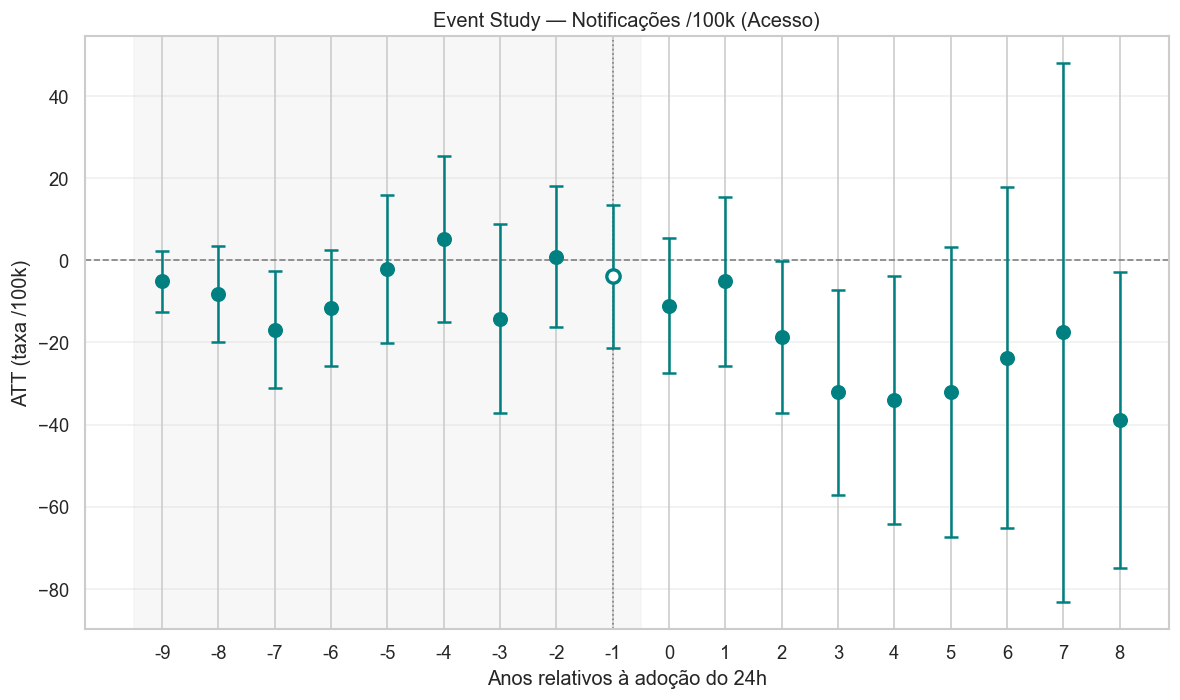
\includegraphics[width=0.49\textwidth]{../figuras_causal/notificacoes_02_event_study.png}\hfill
  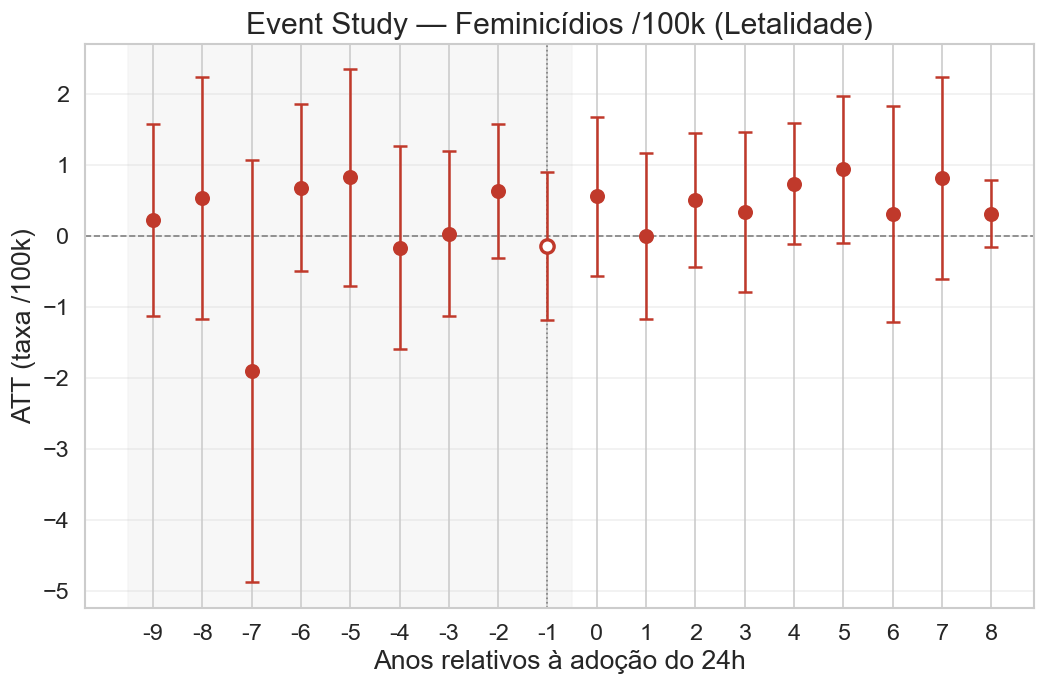
\includegraphics[width=0.49\textwidth]{../figuras_causal/feminicidios_02_event_study.png}
  \caption{Event studies (especificação DR); cada ponto é o $ATT$ no ano relativo
           à adoção do 24h, com IC~95\%. \textbf{Esquerda (Notificações/100k):}
           os coeficientes pré-tratamento ($t<0$) são indistinguíveis de zero
           ($p_{\text{Wald}}=0{,}16$), validando as tendências paralelas; os efeitos
           pós-adoção são sistematicamente negativos. \textbf{Direita (Feminicídios/100k):}
           pré-tendências também satisfeitas ($p_{\text{Wald}}=0{,}21$), com efeitos
           pós-adoção oscilando em torno de zero, sem padrão sistemático, coerente
           com o ATT global não-significativo ($+0{,}48$; ver Seção~\ref{sec:disc}).}
  \label{fig:es}
\end{figure*}

\subsection{Discussão: Causalidade Reversa e Identificação}
\label{sec:disc}

\textbf{O efeito ``positivo'' sobre feminicídios era causalidade reversa.} O
achado central do estudo emerge do contraste entre as duas especificações. Sob
covariáveis de \textit{nível} (porte, renda, violência basal), o ATT de
feminicídios é positivo e \textit{aparentemente} significativo ($+0{,}63$,
$p=0{,}018$), resultado que, lido ingenuamente, sugeriria que a DEAM 24h
\textit{aumenta} feminicídios, uma conclusão tão absurda quanto perigosa. Esse
coeficiente é, na verdade, um artefato de \textbf{causalidade reversa}: gestores
públicos não convertem delegacias aleatoriamente, mas concentram a abertura de
plantões justamente nos municípios onde a violência letal já se encontra em
\textit{viés de alta}, fenômeno conhecido como \textit{reactive policy
adoption}. Os municípios tratados já trilhavam uma trajetória ascendente de
feminicídios no momento da adoção, e o estimador atribuía ao tratamento esse
pico pré-existente.

A correção exigiu a covariável certa. As covariáveis de \textit{nível} não
resolvem o problema, porque ele não é uma diferença de nível, mas uma
\textbf{tendência diferencial}: tratados e controles são quase idênticos em
porte e urbanização, de modo que não há alavancagem para o pareamento. Apenas a
covariável de \textbf{variação} (\texttt{delta\_homicidios\_masc}), que pareia
municípios por surto recente de violência letal, neutraliza a adoção reativa. Com
ela, o efeito encolhe para $+0{,}48$ e perde significância ($p=0{,}064$, IC cruza
zero), e as pré-tendências permanecem satisfeitas. A conclusão honesta é que
\textbf{não há evidência robusta de efeito da DEAM 24h sobre a letalidade}.

\textbf{O princípio metodológico.} O contraste relevante \textit{não} é
``significativo \textit{vs.}\ não-significativo'', e sim \textbf{enviesado
\textit{vs.}\ não-enviesado}. Tendências paralelas é a hipótese de identificação
e precisa valer \textit{independentemente} de o resultado ser significativo;
significância calculada sobre um estimador com pré-tendências violadas não tem
valor inferencial. É por isso que a especificação DR, e não a magnitude ou o
\textit{p}-valor isolados, é o que confere (ou retira) credibilidade aos
resultados.

\textbf{O sinal negativo das notificações.} Já o desfecho de acesso passa a ser
causalmente identificado sob DR (pré-tendências restauradas), mas com sinal
\textbf{negativo} ($-18{,}04$), contrário ao aumento de notificações previsto
pela cadeia causal. Esse resultado pede cautela e permanece em aberto. A hipótese
mais plausível é de \textbf{deslocamento de canal de registro}: o SINAN capta
notificações do sistema de \textit{saúde}, ao passo que a DEAM é um equipamento
\textit{policial}; a abertura do plantão 24h pode redirecionar parte do registro
da violência para o canal policial, reduzindo mecanicamente as notificações de
saúde sem que o acesso institucional efetivo tenha caído. Hipóteses alternativas,
como heterogeneidade entre coortes ou subnotificação diferencial, não podem ser
descartadas com os dados atuais e ficam como agenda. O importante é que o sinal
negativo \textit{não} sustenta a leitura ingênua de que o plantão 24h reduziu o
acesso.

\textbf{Robustez.} Os estimadores alternativos de Sun \& Abraham (2021) e
Borusyak et al.\ (Imputation) não puderam ser computados na especificação DR:
ambos retornam posto deficiente em razão da covariável \texttt{delta\_homicidios\_masc},
ausente nos dois primeiros anos do painel (faltam defasagens). A robustez fica,
portanto, ancorada no próprio contraste base \textit{vs.}\ DR e na estabilidade
das pré-tendências.

\textbf{Escopo dos efeitos: municípios com DEAM única.} Por fim, é preciso
delimitar a que população os efeitos se aplicam. Como detalhado na
Seção~\ref{sec:unidade}, a amostra restringe-se a municípios atendidos por uma
\textit{única} DEAM, condição que torna a data de conversão um evento único e
datável, requisito do desenho escalonado. As grandes metrópoles (São Paulo, Rio
de Janeiro, Belo Horizonte), com redes de várias delegacias convertidas em anos
distintos, foram deliberadamente excluídas para preservar a definição nítida de
tratamento. Os ATTs estimados, tanto o efeito de acesso ($-18{,}04$) quanto o de
letalidade ($+0{,}48$), devem ser lidos, portanto, como o impacto da conversão
em municípios de pequeno e médio porte com uma delegacia especializada. Não é
imediato extrapolá-los para as capitais com redes densas, onde a cobertura 24h é
gradual e parcial, e onde efeitos de transbordamento entre delegacias e de
intensidade de cobertura poderiam operar de modo qualitativamente distinto. A
generalização para esse universo metropolitano fica como agenda, condicionada a
um tratamento explícito da heterogeneidade intramunicipal de cobertura.

% ============================================================
\section{Conclusão}
% ============================================================

\subsection{Síntese dos Achados}

Esta pesquisa realizou a primeira avaliação causal sistemática do impacto da
conversão de DEAMs para regime de plantão 24 horas no Brasil, utilizando o
estimador de Callaway \& Sant'Anna (2021) em sua forma \textbf{duplamente
robusta}, aplicado a um painel balanceado de 285 municípios e 11 anos de dados
(2009--2019). O achado de maior valor é metodológico e substantivo ao mesmo
tempo: o contraste entre a especificação base e a duplamente robusta expõe e
corrige um viés de adoção reativa que, se ignorado, produziria conclusões falsas.

Para o desfecho de letalidade (taxa de feminicídios por 100k habitantes), a
especificação base sugeria um efeito positivo \textit{aparentemente}
significativo que, lido ingenuamente, indicaria que a DEAM 24h aumenta
feminicídios. Ao condicionar na variação recente da violência letal local
(\texttt{delta\_homicidios\_masc}), o efeito encolhe para $+0{,}48$ e perde
significância ($p=0{,}064$, IC~95\% cruzando zero), com pré-tendências
satisfeitas ($p_{\text{Wald}}=0{,}21$). A conclusão honesta é a \textbf{ausência
de evidência robusta} de efeito da política sobre a letalidade: o sinal positivo
da base era \textbf{causalidade reversa} (\textit{reactive policy adoption}), e
não efeito causal.

Para o desfecho de acesso institucional (taxa de notificações por 100k
habitantes), a especificação base violava as tendências paralelas
($p_{\text{Wald}}=0{,}004$), impedindo leitura causal. A especificação DR
\textbf{restaura a validade das pré-tendências} ($p_{\text{Wald}}=0{,}16$) e
identifica um ATT de $-18{,}04$ ($p=0{,}008$). O sinal negativo, contrário ao
esperado, permanece em aberto, sendo o deslocamento do registro do canal de
saúde (SINAN) para o canal policial a hipótese mais plausível.

\subsection{Evidência de Mecanismo: Sazonalidade Horária}

Embora os resultados causais principais exijam cautela interpretativa, a análise
de sazonalidade do SINAN oferece evidência sugestiva do mecanismo causal proposto.
A variável de hora de ocorrência do fato, preenchida em aproximadamente 53\% dos
registros, revela a seguinte distribuição de notificações fora do horário
comercial (08h--17h):

\begin{table}[H]
\centering
\caption{Notificações Fora do Horário Comercial por Grupo e Período}
\label{tab:saz}
\small
\begin{tabular}{@{}lc@{}}
\toprule
\textbf{Grupo / Período} & \textbf{\% fora do hor. comercial} \\
\midrule
Tratados, antes do 24h  & 57,1\% \\
Tratados, após o 24h    & 55,9\% \\
Controles (comercial)    & 57,6\% \\
\bottomrule
\end{tabular}
\smallskip\par
{\footnotesize\sffamily\itshape
Nota: hora refere-se ao momento do fato, não do registro.
Fonte: SINAN/DataSUS.}
\end{table}

Os valores próximos entre os três grupos e períodos sugerem que a \textit{hora
de ocorrência} da violência é relativamente estável: mais de 55\% dos eventos
ocorrem fora do horário comercial em todos os subgrupos. Isso é consistente com
a cadeia causal proposta (há demanda por atendimento noturno), mas indica que a
conversão para 24h não alterou substantivamente o perfil temporal das
\textit{ocorrências registradas}. Uma explicação possível é que o atendimento
24h amplia o volume de notificações, mas não o horário em que as vítimas buscam
registrar a ocorrência, que pode permanecer concentrado no período diurno por
outros motivos (presença de apoio social, deslocamento, crianças na escola etc.).

É importante ressaltar que a hora no SINAN reflete o momento do fato, e não
o momento do registro na delegacia. Portanto, essa análise constitui
\textbf{evidência de mecanismo}, demonstrando que há substantiva violência
fora do horário comercial, e não demonstração direta de impacto no acesso.

Medir diretamente o horário em que as vítimas \textit{buscam} a delegacia
exigiria a hora de registro da ocorrência, informação que não consta do SINAN
e existe apenas nos boletins de ocorrência. Esses registros ficam sob guarda
das Polícias Civis de cada estado, sem base nacional consolidada, de modo que
obtê-los demandaria pedidos formais de acesso em quase todas as unidades da
federação e articulação com órgãos policiais distintos, cada um com seu próprio
sistema e protocolo. Diante desse custo operacional, a extração da hora de
registro foi considerada inviável no escopo deste estudo e descartada,
restando a hora do fato como melhor aproximação disponível do perfil temporal
da demanda.

\subsection{Próximos Passos da Pesquisa}

Com base nos resultados e nas limitações identificadas, os seguintes
desenvolvimentos metodológicos são prioritários:

\begin{enumerate}
  \item \textbf{Validação primária do ano de transição:} O principal vetor de
        erro de medida do estudo está na data de conversão de cada delegacia
        para o regime 24h, hoje levantada por recortes de notícias e diários
        oficiais (Seção~\ref{sec:transicao}). Para reduzir essa imprecisão, é
        possível confirmar a data diretamente na fonte, contatando cada DEAM
        pelos telefones e e-mails do cadastro nacional mantido pela Ouvidoria
        Nacional da Mulher do CNJ (sob supervisão da Conselheira Maria Cristiana
        Ziouva), ou consultando os portais das Polícias Civis estaduais, que
        também divulgam o endereço e os canais de contato de cada delegacia.
        A verificação na fonte permitiria distinguir a data do \textit{anúncio}
        político da data de \textit{efetiva} entrada em operação, corrigindo
        coortes mal datadas e atenuando o viés de atenuação que hoje torna as
        estimativas conservadoras.

  \item \textbf{Fechar a janela do \texttt{delta}:} A covariável de variação é
        nula em 2009--2010 (faltam defasagens, pois a extração de homicídios
        inicia em 2009), enfraquecendo a contribuição das coortes mais antigas
        e impedindo a robustez por Sun \& Abraham e Imputation. Reextrair os
        homicídios de 2007--2008 completaria a série e permitiria reportar esses
        estimadores alternativos sob a especificação DR.

  \item \textbf{Teste de pré-tendências exato:} O teste atual usa a aproximação
        diagonal (soma de $z^2 \sim \chi^2$), que ignora a covariância entre os
        coeficientes. Um teste de Wald completo, com a matriz de variância-
        covariância plena dos coeficientes, daria \textit{p}-valores exatos.

  \item \textbf{Grupo de controle \texttt{not\_yet\_treated}:} A especificação
        atual usa apenas municípios nunca tratados como controle. Uma
        especificação alternativa com \texttt{control\_group='not\_yet\_treated'}
        expande o conjunto de controles válidos para incluir municípios que
        adotarão o 24h no futuro, aumentando a eficiência da estimação.

  \item \textbf{Variáveis raciais:} A incorporação da proporção de mulheres
        negras (pretas + pardas, conforme Estatuto da Igualdade Racial,
        Lei n\textsuperscript{o}~12.288/2010) como interação com o tratamento
        permite avaliar heterogeneidades socioespaciais no impacto da política,
        uma dimensão crítica dadas as desigualdades estruturais de raça no
        acesso à justiça no Brasil.

  \item \textbf{Avaliação da obrigatoriedade legal do 24h:} A
        Lei n\textsuperscript{o}~14.541/2023 tornou obrigatório o funcionamento
        ininterrupto das DEAMs, convertendo o plantão 24h de decisão municipal
        discricionária em norma federal. Com a disponibilização dos microdados de
        mortalidade (SIM) e de notificação (SINAN) posteriores a 2019, em especial
        os de 2023 e 2024, torna-se viável estimar o efeito dessa mudança normativa.
        Por induzir a conversão de um grande número de delegacias em janela estreita,
        a lei configura um choque de política de abrangência nacional que amplia
        substancialmente o grupo tratado e permite reavaliar a cadeia causal sob um
        desenho quase-experimental mais robusto.
\end{enumerate}

\subsection{Implicações para Política Pública}

Mesmo diante das limitações identificadas, os resultados desta pesquisa têm
implicações relevantes para o desenho de políticas públicas de segurança da
mulher. A heterogeneidade substancial dos efeitos por coorte, com as coortes
2016--2017 exibindo ATTs negativos para feminicídios ($-2{,}53$ para coorte
2016; $-1{,}53$ para coorte 2017) e as coortes mais antigas com ATTs positivos,
sugere que a \textbf{maturidade institucional} da DEAM 24h pode ser
determinante para a efetividade da política, ainda que essa leitura deva ser
tomada com cautela dado o ATT global não-significativo. DEAMs convertidas mais
recentemente podem precisar de tempo para desenvolver protocolos de atendimento
noturno, articulação com a rede de proteção e treinamento específico para
os plantões. Essa dinâmica temporal seria invisível num estimador TWFE,
mas emerge claramente na decomposição por coorte do estimador CS DiD.

Para a gestão pública, três recomendações operacionais decorrem da análise.
Primeiro, a avaliação de impacto de plantões 24h deve incorporar explicitamente
o problema da adoção reativa: comparar municípios tratados com controles sem
ajustar para a trajetória prévia de violência produzirá, sistematicamente,
estimativas pessimistas do efeito da política. Segundo, o registro administrativo
padronizado da data de conversão de cada delegacia, hoje inexistente, eliminaria
o erro de medida que atenua os coeficientes e permitiria avaliações mais precisas.
Terceiro, a heterogeneidade por coorte sugere que o monitoramento de efeito deve
respeitar uma janela de maturação institucional, evitando avaliações precoces que
captem apenas a fase de implantação dos protocolos noturnos.

\subsection{Limitações}
\label{sec:limit}

Além das fontes de viés já discutidas, quatro limitações merecem registro.
Primeiro, a covariável de variação (\texttt{delta\_homicidios\_masc}) é nula em
2009--2010 por falta de defasagens, enfraquecendo a contribuição das coortes mais
antigas e impedindo o cálculo dos estimadores de robustez (Sun \& Abraham e
Imputation retornam posto deficiente). Segundo, o teste de pré-tendências usa a
aproximação diagonal de Wald, cujos \textit{p}-valores devem ser lidos como
aproximados. Terceiro, o número reduzido de municípios em algumas coortes (por
exemplo, uma única unidade na coorte de 2009, descartada na especificação DR)
amplia a incerteza dos efeitos por coorte, refletida nos erros-padrão elevados.
Por fim, a amostra limita-se a municípios com uma \textbf{única DEAM}
(Seção~\ref{sec:unidade}): as metrópoles com múltiplas delegacias e anos de
conversão divergentes foram excluídas para manter a definição nítida de
tratamento exigida pelo desenho escalonado. Isso restringe a validade externa
dos achados ao universo de municípios de pequeno e médio porte com uma delegacia
especializada, deixando em aberto o efeito da política nas grandes capitais, onde
a cobertura 24h é parcial e implantada de forma gradual entre unidades.

% ============================================================
% REFERÊNCIAS (não numerada)
% ============================================================
\section*{Referências}
\addcontentsline{toc}{section}{Referências}
\begingroup
\setlength{\parindent}{-0.4cm}
\setlength{\leftskip}{0.4cm}
\setlength{\parskip}{2pt}
\small

\textbf{Bases de Dados}

Base dos Dados. \textit{Sistema de Informações sobre Mortalidade (SIM)}.
Tratamento e disponibilização dos microdados do DataSUS. Disponível em:
\href{https://basedosdados.org/dataset/5beeec93-cbf3-43f6-9eea-9bee6a0d1683?table=dea823a5-cad7-4014-b77c-4aa33b3b0541}{basedosdados.org/dataset/SIM}.
Acesso em: jun. 2026.

Base dos Dados. \textit{Sistema de Informação de Agravos de Notificação
(SINAN)}. Tratamento e disponibilização dos microdados do DataSUS. Disponível em:
\href{https://basedosdados.org/dataset/f51134c2-5ab9-4bbc-882f-f1034603147a?table=7d2d29c1-cfa8-470b-ab13-a83cf522c5ac}{basedosdados.org/dataset/SINAN}.
Acesso em: jun. 2026.

Instituto Brasileiro de Geografia e Estatística — IBGE. \textit{Tabela 6579:
População residente estimada}. SIDRA. Disponível em:
\href{https://sidra.ibge.gov.br/tabela/6579}{https://sidra.ibge.gov.br/tabela/6579}.
Acesso em: jun. 2026.

Instituto Brasileiro de Geografia e Estatística — IBGE. \textit{Tabela 5938:
Produto Interno Bruto a preços correntes} (variável 37). SIDRA. Disponível em:
\href{https://sidra.ibge.gov.br/tabela/5938}{https://sidra.ibge.gov.br/tabela/5938}.
Acesso em: jun. 2026.

\smallskip
\textbf{Referências Metodológicas}

Callaway, B., \& Sant'Anna, P. H. C. (2021). Difference-in-Differences with
multiple time periods. \textit{Journal of Econometrics}, 225(2), 200--230.
\href{https://doi.org/10.1016/j.jeconom.2020.12.001}{https://doi.org/10.1016/j.jeconom.2020.12.001}.

Goodman-Bacon, A. (2021). Difference-in-differences with variation in
treatment timing. \textit{Journal of Econometrics}, 225(2), 254--277.
\href{https://doi.org/10.1016/j.jeconom.2021.03.014}{https://doi.org/10.1016/j.jeconom.2021.03.014}.

Sun, L., \& Abraham, S. (2021). Estimating dynamic treatment effects in
event studies with heterogeneous treatment effects. \textit{Journal of
Econometrics}, 225(2), 175--199.
\href{https://doi.org/10.1016/j.jeconom.2020.09.006}{https://doi.org/10.1016/j.jeconom.2020.09.006}.

Sant'Anna, P. H. C., \& Zhao, J. (2020). Doubly robust difference-in-differences
estimators. \textit{Journal of Econometrics}, 219(1), 101--122.
\href{https://doi.org/10.1016/j.jeconom.2020.06.003}{https://doi.org/10.1016/j.jeconom.2020.06.003}.

\smallskip
\textbf{Literatura Substantiva}

Cerqueira, D., \& Mello, J. M. P. (2012). Menos armas, menos crimes.
\textit{Brazilian Journal of Economics}, 66(1), 29--57.

Lei n\textsuperscript{o}~11.340, de 7 de agosto de 2006. \textit{Lei Maria
da Penha}. Presidência da República, Brasília, DF.
\href{https://www.planalto.gov.br/ccivil_03/_ato2004-2006/2006/lei/l11340.htm}{Texto integral}.

Lei n\textsuperscript{o}~14.541, de 3 de abril de 2023. \textit{Dispõe sobre a
criação e o funcionamento ininterrupto das Delegacias Especializadas de
Atendimento à Mulher}. Presidência da República, Brasília, DF.
\href{https://www.planalto.gov.br/ccivil_03/_ato2023-2026/2023/lei/l14541.htm}{Texto integral}.

Revista AzMina. \textit{Levantamento de Delegacias Especializadas de
Atendimento à Mulher no Brasil}. Curadoria jornalística da rede de atendimento.
Disponível em: \href{https://azmina.com.br}{azmina.com.br}. Acesso em: jun. 2026.

\smallskip
\textbf{Recursos do Projeto}

Santana, F. \textit{Repositório do Projeto DEAM-BR}. GitHub, 2026.
\href{https://github.com/felipesantanafs/deam-br}{https://github.com/felipesantanafs/deam-br}.

Santana, F. \textit{Dashboard Interativo — Avaliação de Impacto das DEAMs 24h}.
Streamlit, 2026.
\href{https://deam-br.streamlit.app}{https://deam-br.streamlit.app}.

\endgroup

\end{document}
